\documentclass[nobib]{tufte-handout}

\title{Lecture 11: Planarity $\cdot$ 1MA020}

\author[Vilhelm Agdur]{Vilhelm Agdur\thanks{\href{mailto:vilhelm.agdur@math.uu.se}{\nolinkurl{vilhelm.agdur@math.uu.se}}}}

\date{22 November 2023}


%\geometry{showframe} % display margins for debugging page layout

\usepackage{graphicx} % allow embedded images
  \setkeys{Gin}{width=\linewidth,totalheight=\textheight,keepaspectratio}
  \graphicspath{{graphics/}} % set of paths to search for images
\usepackage{amsmath}  % extended mathematics
\usepackage{booktabs} % book-quality tables
\usepackage{units}    % non-stacked fractions and better unit spacing
\usepackage{multicol} % multiple column layout facilities
\usepackage{lipsum}   % filler text
\usepackage{fancyvrb} % extended verbatim environments
  \fvset{fontsize=\normalsize}% default font size for fancy-verbatim environments

\usepackage{color,soul} % Highlights for text

% Standardize command font styles and environments
\newcommand{\doccmd}[1]{\texttt{\textbackslash#1}}% command name -- adds backslash automatically
\newcommand{\docopt}[1]{\ensuremath{\langle}\textrm{\textit{#1}}\ensuremath{\rangle}}% optional command argument
\newcommand{\docarg}[1]{\textrm{\textit{#1}}}% (required) command argument
\newcommand{\docenv}[1]{\textsf{#1}}% environment name
\newcommand{\docpkg}[1]{\texttt{#1}}% package name
\newcommand{\doccls}[1]{\texttt{#1}}% document class name
\newcommand{\docclsopt}[1]{\texttt{#1}}% document class option name
\newenvironment{docspec}{\begin{quote}\noindent}{\end{quote}}% command specification environment

\include{mathcommands.extratex}

\begin{document}

\maketitle% this prints the handout title, author, and date

\begin{abstract}
\noindent
We study the notion of a graph being \emph{planar}, define its \emph{planar dual}, and prove some results about when a graph is planar. We give most of a proof of the theorems of Kuratowski and Wagner about forbidden minors for planar graphs.
\end{abstract}

\section{Three-connected graphs}

While the topic of this lecture is planarity, we will need a result about the structure of three-connected graphs. So we begin by proving this.

\begin{figure}
  \centering
  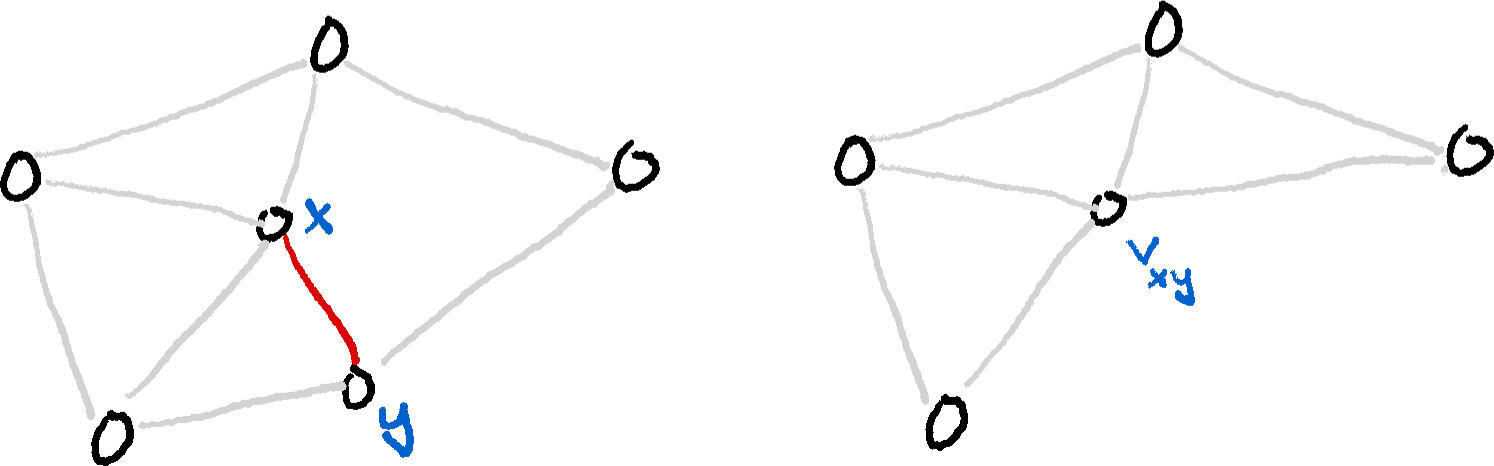
\includegraphics[width=0.75\textwidth]{graphics/L11_planarity/edge_contraction.png}
  \caption[][0cm]{A graph with an edge between $x$ and $y$ highlighted in red. On the right, the result of contracting this edge.}
  \label{fig:edge_contraction}
\end{figure}

\begin{definition}
  Let $G = (V,E)$ be a graph and $e = x\sim y$ be an edge of $G$. The \emph{contraction} of $e$ is the graph $G/e$, which we construct as follows:

  Introduce a new vertex $v_{xy}$, and let $V(G/e) = (V \setminus \{x,y\}) \cup \{v_{xy}\}$. Replace each edge $w \sim x$ or $w \sim y$ with an edge $w \sim v_{xy}$.
\end{definition}

\begin{lemma}\label{lemma:existence_of_contraction_edge}
  If $G = (V,E)$ is three-connected and has more than four vertices, then there exists an edge $e \in E$ such that $G/e$ is again three-connected.

  \begin{proof}
    Suppose there is no such edge, so that for every edge $e = x \sim y$ there is a separating set $X$ of $G/e$ on two or fewer vertices. Now, since $G$ is three-connected, we must in fact have $X = \{v_{xy}, z\}$.

    Then the set $\{x, y, z\}$ must be a separating set for $G$. Each of these three vertices must have a neighbour in every connected component of $G[V \setminus \{x,y,z\}]$.\sidenote[][]{
      \begin{xca}
        Prove this.
      \end{xca}
    } Let $C$ be the smallest such component, and further assume we chose $x$, $y$, and $z$ in such a way that $\abs{V(C)}$ was minimal across all choices.

    Now, choose a neighbour $v$ of $z$ in $C$. By our assumption, no edge-contracton is three-connected, so in particular $G/(v \sim z)$ is not three-connected. By entirely the same argument as before, we can find a vertex $w$ such that $\{z,v,w\}$ separates $G$.

    Again, each of $z$, $v$, and $w$ has a neighbour in each connected component of $G[V \setminus \{z, v, w\}]$. Since there is an edge between $x$ and $y$, they must be in the same component, and so there is a component $D$ which contains neither. Since $v \in C$, each of its neighbours is also in $C$, and so in particular is its neighbour in $D$.

    So $D \cap C \neq \emptyset$. Since $D$ does not contain any of $x$, $y$, or $z$, their removal can't disconnect $D$, and so it follows from this that $D \subseteq C$. However, $D$ clearly does not contain $v$, being a connected component of $G[V \setminus \{z, v, w\}]$, while $C$ does contain $v$. So $D$ is in fact strictly smaller than $C$, which is a contradiction, since we assumed $C$ was minimal. So the lemma follows.
  \end{proof}
\end{lemma}

We also state, but do not prove, a classification of the three-connected graphs, due to Tutte. It is in some sense analogous to our theorem about two-connected graphs being constructible by adding paths to a cycle graph.

\begin{theorem}[Tutte, 1961]
  A graph $G$ is three-connected if and only if there exists a sequence $G_0, G_1,\ldots, G_n$ of graphs, where $G_0 = K_4$, $G_n = G$, and for every $i \in [n]$ the graph $G_i$ has an edge $u \sim v$ with $d_{G_i}(u), d_{G_i}(v) \geq 3$ and $G_{i-1} = G_i/(u\sim v)$.
\end{theorem}

\section{Planarity}

One way to think about the notion of planarity is that we want to study graphs arising from maps, as we saw in the exercise session. Another might be that we just want to find nice ways to draw graphs. Let us give a not very precise definition of what we mean by drawing a graph:

\begin{definition}
  A \emph{drawing} or \emph{embedding} of a graph in $\R^2$ is a way of placing all the vertices of the graph at distinct points, and drawing an arc\sidenote[][]{In a more precise definition we would have to state what we assume about these arcs -- are they continuous, smooth, piecewise linear?} between any two adjacent vertices.

  We say that an embedding is \emph{planar}, and call the embedded graph a \emph{plane} graph, if this can be done so that none of the edges intersect.
\end{definition}

\begin{definition}
  Any planar embedding of a graph divides the plane into several connected components, called \emph{faces}. Exactly one of these faces is unbounded, and any other faces are bounded.\sidenote[][]{In order to prove this you need the seemingly obvious but surprisingly hard-to-prove Jordan curve theorem.}

  Generally, any cycle $C$ in a plane graph $G = (V,E)$ will separate the vertices of $G$ into three sets,
  $$V = O \amalg V(C) \amalg I,$$
  where $O$ are the vertices outside the cycle and $I$ the vertices inside the circle. There are no edges between the sets $O$ and $I$.
\end{definition}

Now we can give a definition of the notion of planar dual, which we introduced in the exercises:

\begin{definition}
  Let $G = (V,E)$ be a plane graph, that is, a planar graph with a given embedding. The \emph{planar dual} $G^* = (F, E^*)$ of $G$ is the multigraph whose vertices are the faces of the embedding of $G$, and where we draw an edge between two faces $f$ and $f'$ if they border each other.

  There is a natural one-to-one correspondence between $E$ and $E^*$ by sending each edge $e\in E$ to the edge between the two faces it separates.

  See Figure \ref{fig:planar_dual} for an illustration of this.
\end{definition}

\begin{figure}
  \centering
  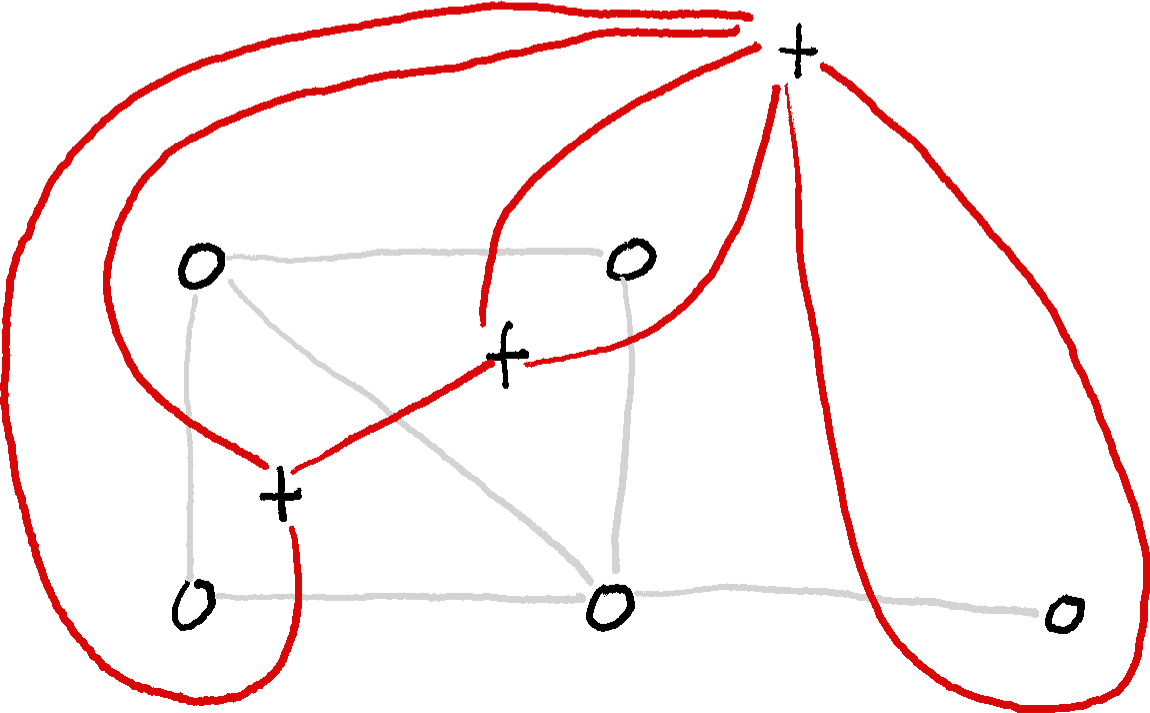
\includegraphics[width=0.65\textwidth]{graphics/L11_planarity/planar_dual.png}
  \caption[][0cm]{A plane graph, with circular black vertices and grey edges, and its planar dual, with black crosses as vertices and red edges. Notice how the correspondence between $E$ and $E^*$ is on display here -- each red edge intersects precisely one grey edge, and vice versa.}
  \label{fig:planar_dual}
\end{figure}

Next, let us prove a theorem about what is often referred to as Euler's formula, though Euler in fact did not think about this for graphs but for polyhedra.

\begin{theorem}[Euler's formula]
  Let $G = (V,E)$ be a connected planar graph, and let $f$ be the number of faces for some planar embedding of $G$. Then\sidenote[][]{The thing on the left-hand side here is called the \emph{Euler characteristic}, which is the first step on a long journey of geometry and the genus of surfaces. If you want a book-length discussion of the history of this formula, and the history of the notion of mathematical proof in general, read Imre Lakatos \emph{Proofs and Refutations}.}
  $$\abs{V} - \abs{E} + f = 2,$$
  and so in particular any two planar embeddings have the same number of faces.

  \begin{definition}
    Let $G = (V,E)$ be a connected planar graph, fix a planar embedding of it, and construct its planar dual $G^* = (F, E^*)$. Next, fix a spanning tree $T = (V, E_T)$ of $G$, and consider its complement in the planar dual, $T* = (F, E^* \setminus E_T)$.

    Now, let us show that this $T^*$ is in fact a tree.\sidenote[][]{We already showed this in the exercise session, but let us repeat ourselves.} If $T^*$ were disconnected, one of its connected components would not contain the unbounded face, and this set of faces would be enclosed by a cycle of $T$. But $T$ has no cycles, since it is a tree.

    If $T^*$ contained a cycle, this cycle would necessarily enclose a vertex of $T$, which would be separated from the rest of $T$, and so $T$ would be disconnected, which is again impossible since $T$ is a tree.

    So, we have seen that $T$ is a tree on $\abs{V}$ vertices and thus has $\abs{V} - 1$ edges, and $T^*$ is a tree on $\abs{F}$ vertices and thus $\abs{F}-1$ edges. However, since $T^*$ has as its edges the complement of the edges of $T$, they must together have $\abs{E}$ edges. So we have shown that
    $$\left(\abs{V} - 1\right) + \left(\abs{F} - 1\right) = \abs{E},$$
    which rearranges to show the theorem.
  \end{definition}
\end{theorem}

It is easy to see how one might show a graph is planar -- just find a planar embedding of it. How do you prove a graph is \emph{not} planar? It is not immediately obvious how one would do that, other than by somehow considering every embedding and finding a pair of edges which intersect.

So we are interested in simpler ways to prove that a graph is not planar. Our first method is just a corollary of Euler's formula.

\begin{corollary}
  If $G = (V,E)$ is a planar graph on at least three vertices, then
  $$\abs{E} \leq 3\abs{V} - 6.$$

  If it additionally does not contain a triangle, then
  $$\abs{E} \leq 2\abs{V} - 4.$$

  \begin{proof}
    We will prove this by a double counting argument. The thing we will count is the number pairs of an edge and a face it is incident to, counting with multiplicity.\sidenote[][]{So, for a $K_2$, its one edge is incident to the single face twice, once per side of the edge.}

    On the one hand, clearly, each edge is incident two two faces, so the total is $2\abs{E}$. On the other hand, each face clearly has at least three edges incident to it, so the the total is at least $3\abs{F}$.

    So we have seen that $3\abs{F} \leq 2\abs{E}$, which together with Euler's formula gives the result. If $G$ additionally contains no triangles, then of course each face is incident to at least \emph{four} edges,\sidenote[][]{You see here how we could get an entire family of results, by assuming that $G$ has no cycles of length less than $k$ for varying $k$. The length of the shortest cycle in a graph is its \emph{girth}, as we shall see in our next lecture.} giving us instead $4\abs{F} \leq 2\abs{E}$, which together with Euler's formula rearranges to the stronger result.
  \end{proof}
\end{corollary}

\begin{corollary}
  The graphs $K_5$ and $K_{3,3}$ are non-planar.

  \begin{proof}
    For $K_5$, it follows by the first part of the previous corollary. $K_{3,3}$ is of course bipartite, and so in particular contains no triangles, and so it follows for this graph by the second part of the corollary.
  \end{proof}
\end{corollary}

So we have shown two graphs to be non-planar. This in fact gives us a more general method to see that a graph is non-planar: If it contains a subgraph isomorphic to $K_5$ or to $K_{3,3}$ it cannot be planar, since already that subgraph can't be embedded without edges crossing, and adding more edges and vertices certainly won't change that.

It turns out that in fact this classifies exactly which graphs are non-planar, if we expand our notion of ``containing'' from just ``having a subgraph'' to the notion of a \emph{minor}.

\begin{definition}
  Let $G$ and $H$ be graphs. A \emph{subdivision} of $H$ is a graph where some of the edges of $H$ were replaced by paths. If a graph $G$ contains a subdivision of $H$,\sidenote[][]{That is, has a subgraph isomorphic to a subdivision of $H$.} then $H$ is a \emph{topological minor} of $G$.
\end{definition}

It should be intuitively clear that a subdivision of $H$ is planar if and only if $H$ is, so the operation of taking subdivisions doesn't affect planarity. So if a graph has a topological minor that is non-planar, then it itself is also non-planar.

There is also a second notion of minor, which is what we normally mean by being a minor:

\begin{definition}
  Let $G$ and $H$ be graphs. $H$ is a \emph{minor} of $G$ if there is a subgraph $G'$ of $G$ such that $H$ can be obtained from $G'$ by a sequence of edge-contractions. Equivalently, $H$ is a minor of $G$ if it can be obtained from $G$ by deleting vertices or edges and contracting edges.
\end{definition}

If you think about it for a bit, it should be clear that it is also true that having a minor in this sense that is non-planar means you cannot yourself be planar.

So, a graph that has a $K_5$ or a $K_{3,3}$ as a minor or topological minor cannot be planar. In fact, it turns out that the converse is also true -- any non-planar graph has one of them as a minor and as a topological minor. This is the content of the theorems of Kuratowski and Wagner:

\begin{theorem}[Kuratowski, 1930]
  A graph is planar if and only if it contains neither a $K_5$ nor a $K_{3,3}$ as a topological minor.
\end{theorem}

\begin{theorem}[Wagner, 1937]
  A graph is planar if and only if it contains neither a $K_5$ nor a $K_{3,3}$ as a minor.
\end{theorem}

The proof of the hard direction of this theorem is in three steps, of which we will only do the second:
\begin{enumerate}
  \item Show that a graph contains one of $K_{5}$ or $K_{3,3}$ as a topological minor if and only if it contains one of them as a minor.\sidenote[][]{This is Proposition 1.7.3 and Lemma 4.4.2 in the book by Diestel, if you want to see a proof -- or just Google for it.}
  \item One proves that any three-connected graph which does not contain $K_5$ or $K_{3,3}$ as a minor is planar.
  \item Finally, we show that the edge-maximal graphs without $K_5$ or $K_{3,3}$ as a topological minor are three-connected.\sidenote[][]{Which is the content of Lemmas 4.4.4 and 4.4.5 in the Diestel book.} The idea then is that given any graph $G$ not containing the forbidden minors, you can add edges avoiding creating a $K_5$ or $K_{3,3}$ until it is maximal, and it will then be three-connected without those minors, which by the previous step implies that it is planar. Then of course any subgraph of it is also planar, and so in particular the $G$ you started with is planar.
\end{enumerate}

Having seen the overall structure of the proof, let us actually do a proof of the second step:

\begin{lemma}
  Let $G = (V,E)$ be a three-connected graph without a $K_5$ or a $K_{3,3}$ as a minor. Then $G$ is planar.

  \begin{proof}
    We prove this by induction in the number of vertices. The smallest three-connected graph is a $K_4$, and this one is evidently planar and has no such minors.

    So assume $\abs{V} > 4$ and that the claim holds for all graphs on fewer vertices. Since $G$ is three-connected on more than four vertices, it follows from Lemma \ref{lemma:existence_of_contraction_edge} that there exists an edge $e = \{x,y\}$ in $G$ such that the contraction $G/e$ is again three-connected.

    Now, this $G/e$ is a minor of $G$, and hence it can't contain a $K_5$ or $K_{3,3}$ minor.\sidenote[][]{This follows from the fact that being a minor is a transitive relation -- if $G$ is a minor of $G'$ and $G'$ a minor of $G''$, then $G$ is a minor of $G''$.} So by our induction hypothesis, $G/e$ is planar.

    Now, consider a planar embedding of $G/e$. If we remove the vertex $v_{xy}$, the one we got by contracting the edge $x\sim y$, we again get a plane graph, and in this drawing of $G/e - v_{xy}$ there is one face that used to contain $v_{xy}$. Since $G/e$ is three-connected, the boundary of this face is a cycle $C$.\sidenote[][]{Why do we need three-connectedness here?}

    \begin{figure}
      \centering
      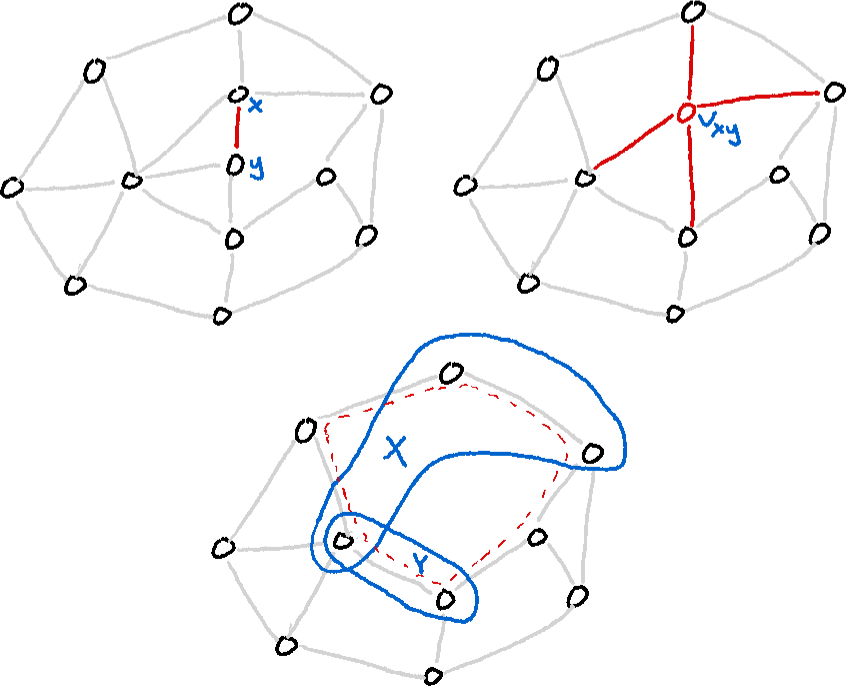
\includegraphics[width=0.7\textwidth]{graphics/L11_planarity/wagner_kuratowski_proof.png}
      \caption[][0cm]{Top left, a three-connected graph with an edge $x\sim y$ highlighted. Top right, another graph which is the result of contracting this edge, with the new edges and vertices in red. Bottom, the result of removing the contraction vertex $v_{xy}$, with the face on which it sat indicated by a dotted red line, which is also the cycle $C$, and the sets $X$ and $Y$ indicated.}
      \label{fig:wagner_kuratowski}
    \end{figure}

    Let $X = N(x)\setminus \{y\}$ be the set of neighbours of $x$ other than $y$, and likewise let $Y = N(y) \setminus \{x\}$. Notice how $X$ and $Y$ are both subsets of the cycle $C$.

    Now, if we take our embedding of $G/e$ and remove all edges $v_{xy}\sim w$ for $w \in Y \setminus X$, we get an embedding of the graph $G[V\setminus\{y\}]$, with the vertex $v_{xy}$ replacing $x$. So if we can find a way to add $y$ back into this drawing, then we will have a planar embedding of $G$.

    So, number the vertices of $X$ as $x_1, x_2, \ldots, x_r$ in clockwise order around the cycle $C$, and notice that they partition the cycle $C$ into paths $P_i$ from $x_i$ to $x_{i+1}$, as in Figure \ref{fig:w_k_cycle}.

    \begin{figure}
      \centering
      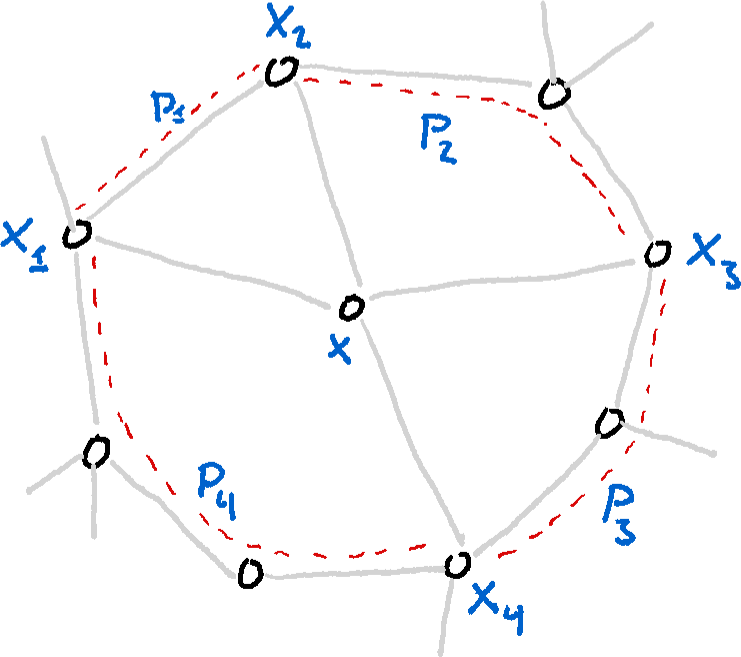
\includegraphics[width=0.6\textwidth]{graphics/L11_planarity/w_k_cycle.png}
      \caption[][0cm]{A local picture of the embedding of $G[V\setminus\{y\}]$, with the vertices of $X$ labelled, and the paths between in dashed red lines.}
      \label{fig:w_k_cycle}
    \end{figure}

    If we could show that all the vertices of $Y$ lie on the same path $P_i$, then we could add $y$ back into the drawing by adding to the face bounded by this path and the edges between it and $x$.

    So suppose for contradiction that not all neighbours of $y$ lie on the same path $P_i$. There are three cases:\sidenote[][-1.5cm]{These are exhaustive, but not mutually exclusive.}

    \begin{marginfigure}
      \centering
      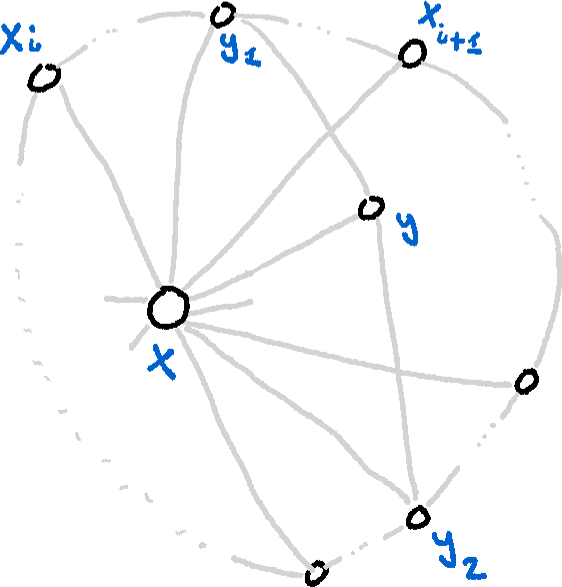
\includegraphics[width=0.75\textwidth]{graphics/L11_planarity/w_k_case1.png}
      \caption[]{A drawing of the first case in our case analysis.}
      \label{fig:w_k_case1}
    \end{marginfigure}

    \begin{enumerate}
      \item Suppose $y_1 \in Y \setminus X$ lies on the interior of some $P_i$, and there is a $y_2 \in Y$ that is not on $P_i$. Then $\{x, y_1, y_2\}$ and $\{y, x_i, x_{i+1}\}$ form the vertices of a topological $K_{3,3}$. This is illustrated in Figure \ref{fig:w_k_case1}.
      \begin{marginfigure}
        \centering
        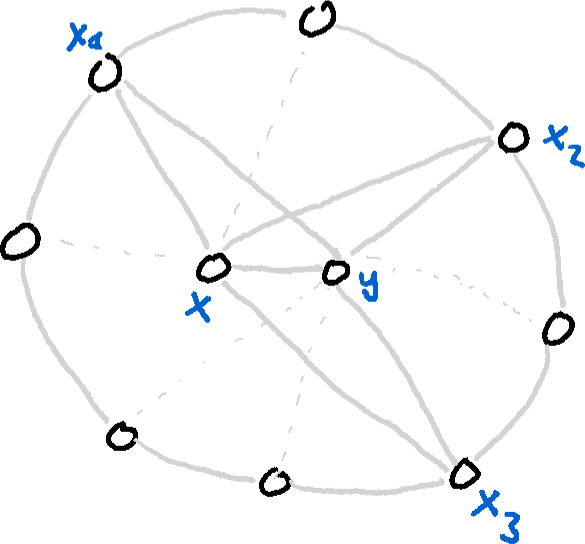
\includegraphics[width=0.75\textwidth]{graphics/L11_planarity/w_k_case2.png}
        \caption[]{A drawing of the second case in our case analysis.}
        \label{fig:w_k_case2}
      \end{marginfigure}
      \item Suppose that $X \cap Y$ has more than two elements -- say $x_i, x_j, x_k$. But then $\{x, y, x_i, x_j, x_k\}$ forms the vertex set of a topological $K_5$. This is illustrated in Figure \ref{fig:w_k_case2}.
      \begin{marginfigure}
        \centering
        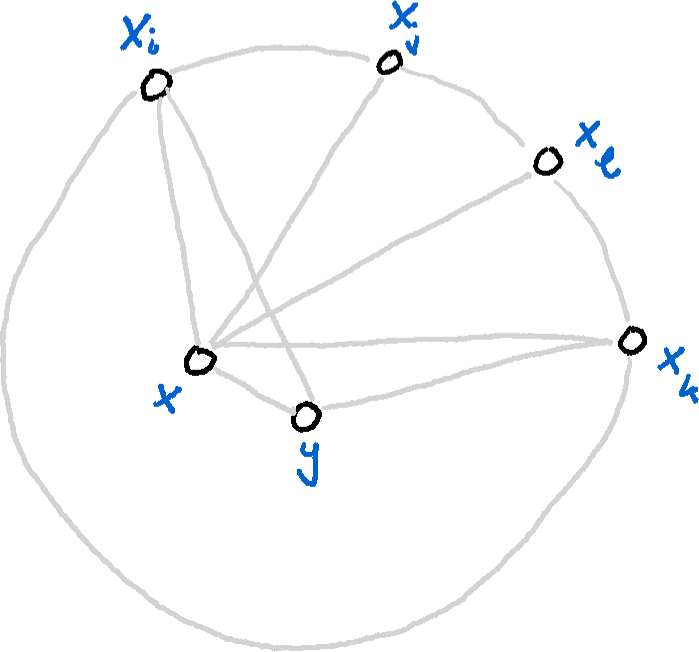
\includegraphics[width=0.75\textwidth]{graphics/L11_planarity/w_k_case3.png}
        \caption[]{A drawing of the third case in our case analysis.}
        \label{fig:w_k_case3}
      \end{marginfigure}
      \item If neither of the above two cases occurs, but $y$ still has neighbours that do not share a path, we must have that $y$ has two neighbours shared with $x$, say $x_i$ and $x_k$, which do not lie on a common path. Then there must be vertices $x_j$ and $x_\ell$ between them. Now $\{x_i, x, x_k\}$ and $\{x_j, y, x_\ell\}$ form the vertices of a topological $K_{3,3}$. This is illustrated in Figure \ref{fig:w_k_case3}.
    \end{enumerate}

    So we have seen that all neighbours of $y$ other than $x$ share a path, and so we can draw $y$ into the corresponding face, getting a planar embedding of the entire graph $G$.
  \end{proof}
\end{lemma}

\section{Exercises}


%\bibliography{references}
%\bibliographystyle{plainnat}

\end{document}
